%!TEX root = <../index.tex>

\section{Experimental Results and Discussion}
\label{sec:5}

The experimental results are described, analyzed and concluded in this section. In section \ref{sec:5.1} the statistics of the corpus after preprocessing is showed briefly. Section \ref{sec:5.2} focuses on the effectiveness of the different STS models, i.e. how precise the STS models predicts an articles as related for a given target article. Furthermore, the operational performance of the STS models is reported in section \ref{sec:5.3}. The above three parts concentrate on the first experiment, which is mentioned in section \ref{sec:4.4}. On the next step, the results of the second experiment are reported in section \ref{sec:5.4}. After reporting the results of the both experiments, we discuss the most severe types of errors that an articles which is virtually unrelated is predicted as related for a target article or a cluster of articles which are properly related are never or rarely predicted as related. In conclusion, we summarize the consequence of selection of the STS models and the challenge of the current work. 

\subsection{Analysis of Preprocessing}
\label{sec:5.1}

Each article contains three semantic components including \ititle{}, \ititle{}, \isummary{} which are as input data of the framework. These components are also called data sources. After preprocessing the data sources in raw string format is converted to a sequence of phrases which consist of $n$ tokens. For the n-gram model with different value of $n = 1, 2, 3$, we have three different representation forms for every data source. A vocabulary is generated from all converted by preprocessing methods data for each representation form of each data source.

\begin{figure}[!htb]
    \centering
    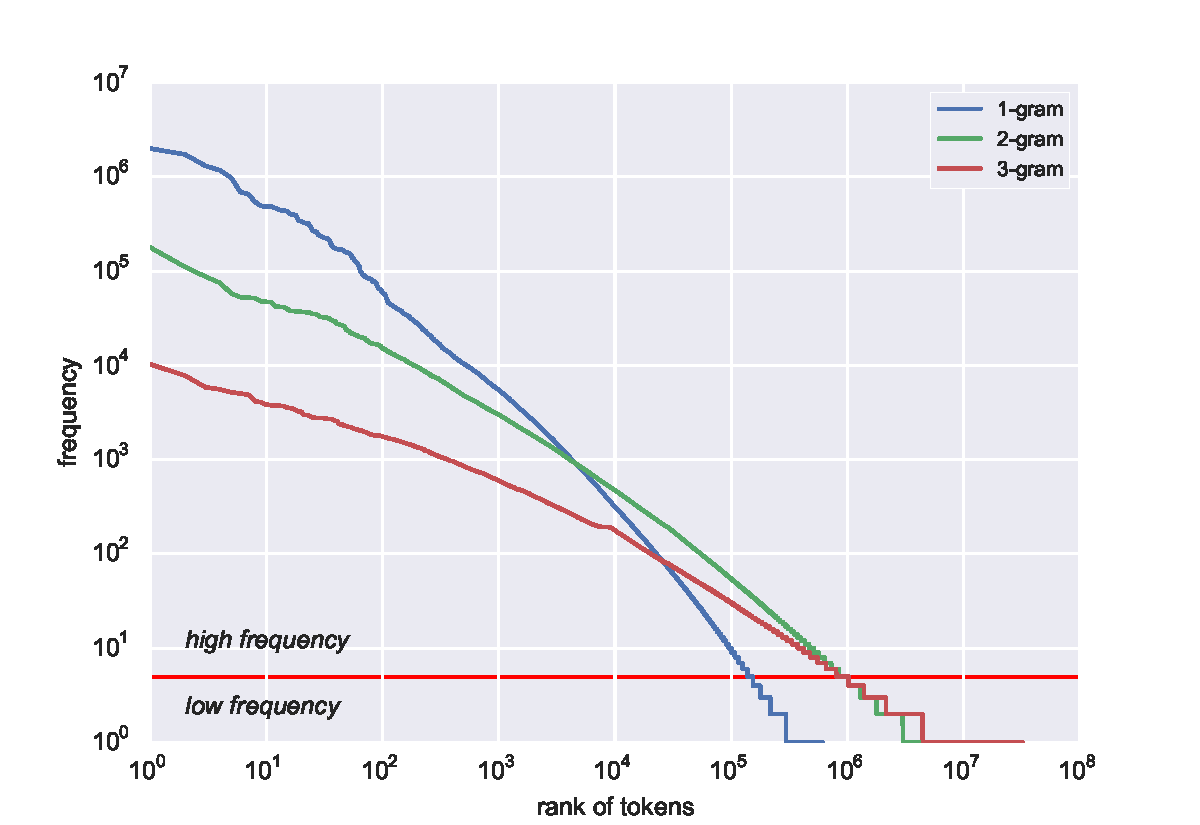
\includegraphics[width=0.8\textwidth]{fig/freqdist}
    \caption{Occurrence Frequency of terms in the corpus for uni-, bi- and trigram in descend ranking. The corresponding preprocessing is \iSE{} and the data source is \icontent{}.}
    \label{fig:freqdist}
\end{figure}

There are two main metrics to portray a vocabulary. The first metric is the size, which impacts the complexity of computing in next phases of discovering related articles. The second one is the scale of long tail of the vocabulary. According to the Zipf's law, the occurrence frequency is distributed extremely unevenly or that is to say that the most terms occur rarely in use and hence it is almost incapable to determine the semantic relevance of these terms by statistical methods. In ideal case, a vocabulary with smaller size and fewer not common used terms has the better quality with both of operational complexity and semantic completeness. Figure \ref{fig:freqdist}, which depicts a representative sample the distribution of the occurrence frequency, indicates that only a small quantity of tokens occur repetitively in the corpus (25\% for unigram, 10\% for bigram and 3\% for trigram). Taking into account efficiency, the tokens which appear less than $5$ times can be removed from the vocabulary. We denote the original vocabularies as \ifull{} vocabularies and the reduced vocabularies as \icommon{} vocabularies. 

\begin{figure}[!htb]
    \centering
    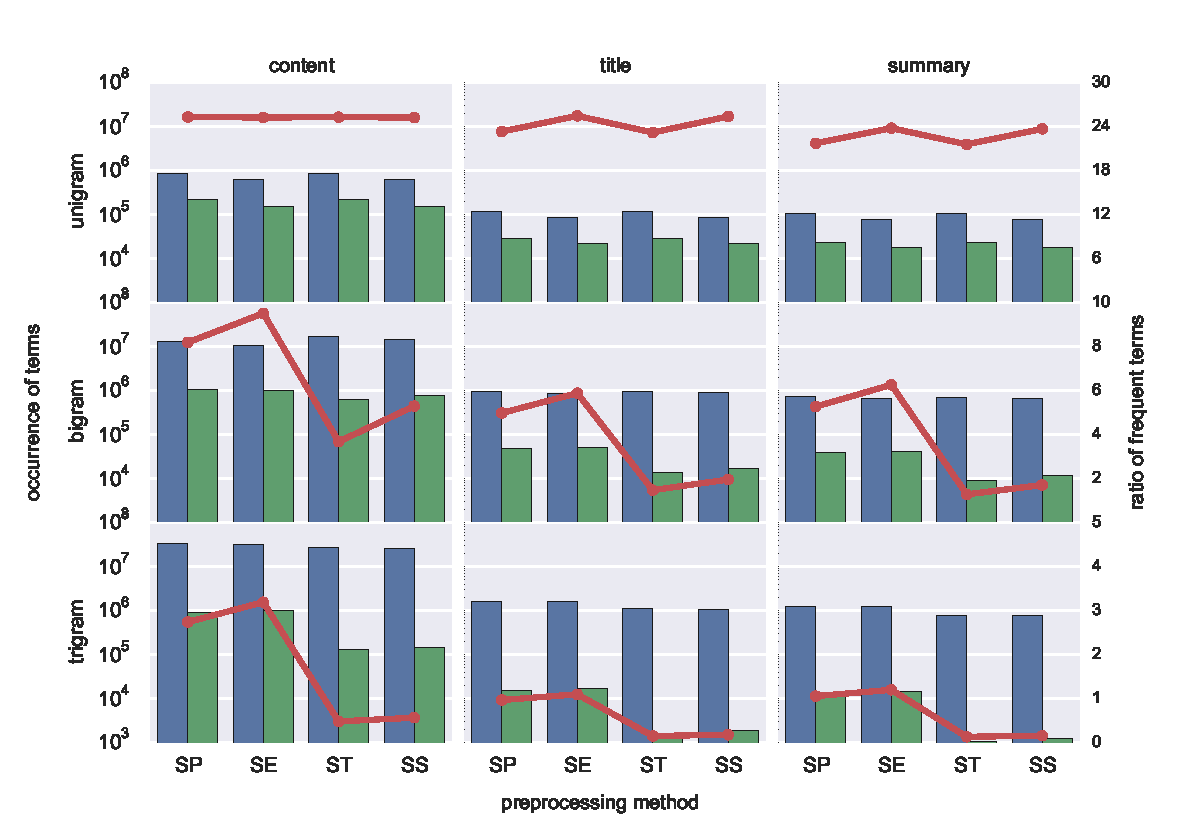
\includegraphics[width=\textwidth]{fig/vocab_size}
    \caption{Comparison the vocabulary size of different preprocessing methods for given data sources with n-gram models. Each column refers to a kind of data source, which is \icontent{}, \ititle{} and \isummary{} respectively while each row refers to a n-gram model: uni-, bi-, and trigram. \textit{Full} vocabularies are illustrated as blue bars and \icommon{} vocabularies as green bars. The red line shows the ratio of the size of \icommon{} vocabularies to the corresponding \ifull{} vocabularies. }
    \label{fig:vocab_size}
\end{figure}


We consider the size of \ifull{} vocabularies and the proportion of frequent tokens as the metrics to evaluate the vocabulary quality. Figure \ref{fig:vocab_size} shows the comparison between the size of \ifull{} and \icommon{} vocabularies which are generated by the preprocessing methods including \iSP{}, \iSE{}, \iST{} and \iSS{} in the different n-gram models ($n=1, 2, 3$) of the three kinds of data source containing \icontent{}, \ititle{} and \isummary{}. In the unigram model, \iSS{} always generates the both smallest vocabularies with the largest proportion of frequent terms. In bi- and trigram, the vocabularies generated by \iSE{} has the largest proportion of frequent terms and the size is slightly different with the vocabularies generated by other methods. In conclusion, the preprocessing method \iSS{} is applied in unigram and \iSE{} is applied in both of bigram and trigram. 


\subsection{Effectiveness of STS Models}
\label{sec:5.2}

As described in section \ref{sec:3.3}, the effectiveness metrics include \textit{precision@k@h} to evaluate the relatedness of the articles of top ranking and \textit{nDCG} to evaluate the overall results. First, the results for each data source with n-gram are given and the best STS models is selected respectively. We give a reasonable assumption that an article is related to the articles which are not farther than $3$ hops. In order to analyze the effectiveness, the assumption is relaxed or that is to say, that the effectiveness is evaluated in the cases of $1$-hop, $3$-hops, $5$-hops and $10$-hops. In the end of the section, the divergence between different categories is discussed and which categories the framework is more suitable for are concluded.  

\subsubsection{Model Selection}



\begin{table}[]
\centering
\begin{tabular}{lllrl}
\hline
source & n-gram & model & \multicolumn{1}{l}{precision} & nDCG \\ \hline
\multirow{13}{*}{Content} & \multirow{5}{*}{unigram} & \textbf{tfidf} & \textbf{0.45} &  \\
 &  & bow & 0.40 &  \\
 &  & jaccard & 0.39 &  \\
 &  & lsi & 0.39 &  \\
 &  & lda & 0.16 &  \\ \cline{2-5} 
 & \multirow{4}{*}{bigram} & \textbf{tfidf} & \textbf{0.43} & \textbf{} \\
 &  & jaccard & 0.36 &  \\
 &  & lsi & 0.27 &  \\
 &  & bow & 0.26 &  \\ \cline{2-5} 
 & \multirow{4}{*}{trigram} & \textbf{tfidf} & \textbf{0.29} & \textbf{} \\
 &  & jaccard & 0.29 &  \\
 &  & bow & 0.23 &  \\
 &  & lsi & 0.14 &  \\ \hline
\multirow{13}{*}{title} & \multirow{5}{*}{unigram} & \textbf{tfidf} & \textbf{0.31} & \textbf{} \\
 &  & bow & 0.28 &  \\
 &  & jaccard & 0.25 &  \\
 &  & lsi & 0.14 &  \\
 &  & lda & 0.10 &  \\ \cline{2-5} 
 & \multirow{4}{*}{bigram} & \textbf{tfidf} & \textbf{0.12} & \textbf{} \\
 &  & jaccard & 0.12 &  \\
 &  & bow & 0.09 &  \\
 &  & lsi & 0.03 &  \\ \cline{2-5} 
 & \multirow{4}{*}{trigram} & \textbf{jaccard} & \textbf{0.09} & \textbf{} \\
 &  & tfidf & 0.04 &  \\
 &  & bow & 0.04 &  \\
 &  & lsi & 0.03 &  \\ \hline
\multirow{13}{*}{summary} & \multirow{5}{*}{unigram} & \textbf{tfidf} & \textbf{0.21} & \textbf{} \\
 &  & jaccard & 0.17 &  \\
 &  & bow & 0.14 &  \\
 &  & lsi & 0.05 &  \\
 &  & lda & 0.05 &  \\ \cline{2-5} 
 & \multirow{4}{*}{bigram} & \textbf{jaccard} & \textbf{0.08} & \textbf{} \\
 &  & tfidf & 0.06 &  \\
 &  & bow & 0.04 &  \\
 &  & lsi & 0.01 &  \\ \cline{2-5} 
 & \multirow{4}{*}{trigram} & \textbf{jaccard} & \textbf{0.06} & \textbf{} \\
 &  & bow & 0.03 &  \\
 &  & tfidf & 0.03 &  \\
 &  & lsi & 0.03 &  \\ \hline
\end{tabular}
\caption{My caption}
\label{my-label}
\end{table}


\subsubsection{Precision from $1$-hop to $10$-hops}

\subsubsection{Divergence between Categories}



\subsection{Efficiency of STS Models}
\label{sec:5.3}

\subsection{Results of Incremental Updating}
\label{sec:5.4}

\subsubsection{Effectiveness}

\subsubsection{Efficiency}

\subsection{Error Analysis}
\label{sec:5.5}

\subsection{Conclusion}
\label{sec:5.6}
